\section{System Architecture: OpenAlex Global AI Dashboard}

\subsection{Project Overview}

The OpenAlex Global AI Dashboard is a comprehensive data visualization and analysis system designed to track global research trends in Artificial Intelligence and Deep Learning from 2010--2020. The system combines real-time API integration with static data analysis to provide both live querying capabilities and historical trend analysis.

\subsection{Complete Project Structure}

The project follows a modular architecture with clear separation of concerns:

\subsection{System Architecture Diagram}

The following diagram illustrates the complete data flow architecture of the system:

\begin{figure}[h]
\centering
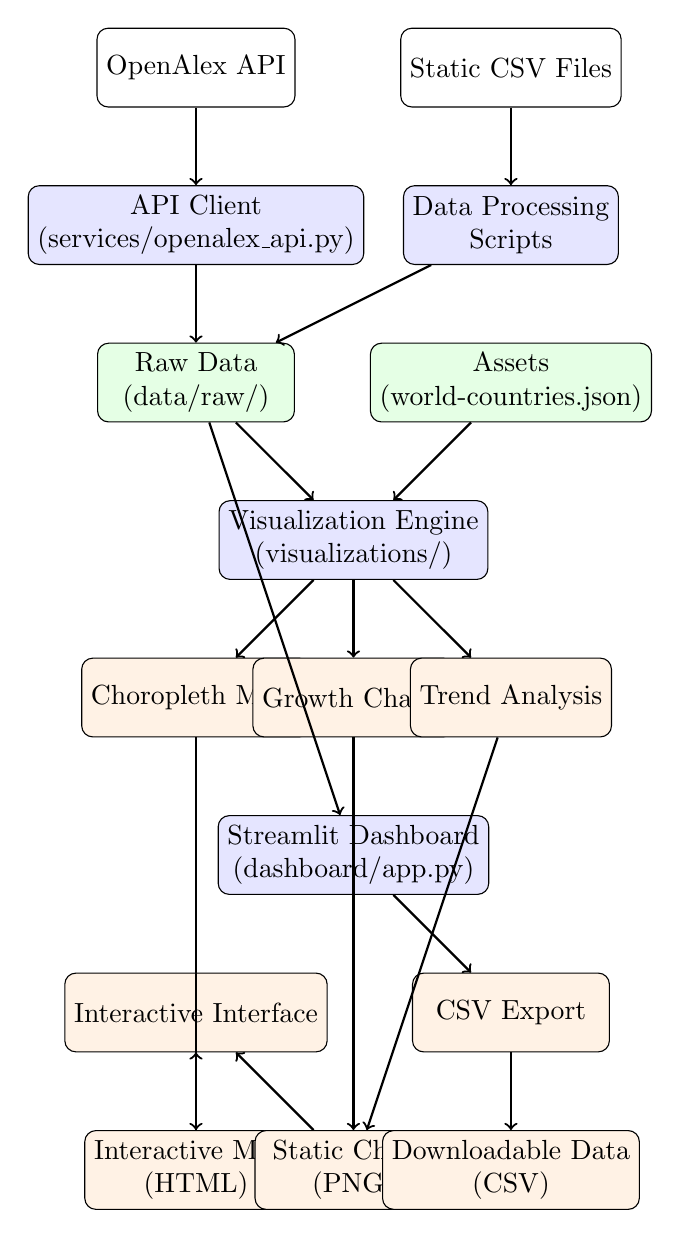
\begin{tikzpicture}[
    node distance=1.5cm,
    box/.style={rectangle, draw, rounded corners, minimum width=2.5cm, minimum height=1cm, align=center},
    process/.style={rectangle, draw, rounded corners, minimum width=2.5cm, minimum height=1cm, align=center, fill=blue!10},
    storage/.style={rectangle, draw, rounded corners, minimum width=2.5cm, minimum height=1cm, align=center, fill=green!10},
    output/.style={rectangle, draw, rounded corners, minimum width=2.5cm, minimum height=1cm, align=center, fill=orange!10},
    arrow/.style={->, thick}
]

% Data Sources
\node[box] (oa) at (0,0) {OpenAlex API};
\node[box] (csv) at (4,0) {Static CSV Files};

% Data Processing Layer
\node[process] (api) at (0,-2) {API Client\\(services/openalex\_api.py)};
\node[process] (proc) at (4,-2) {Data Processing\\Scripts};

% Data Storage
\node[storage] (raw) at (0,-4) {Raw Data\\(data/raw/)};
\node[storage] (assets) at (4,-4) {Assets\\(world-countries.json)};

% Visualization Engine
\node[process] (viz) at (2,-6) {Visualization Engine\\(visualizations/)};
\node[output] (maps) at (0,-8) {Choropleth Maps};
\node[output] (charts) at (2,-8) {Growth Charts};
\node[output] (trends) at (4,-8) {Trend Analysis};

% Web Application
\node[process] (streamlit) at (2,-10) {Streamlit Dashboard\\(dashboard/app.py)};
\node[output] (ui) at (0,-12) {Interactive Interface};
\node[output] (export) at (4,-12) {CSV Export};

% Output
\node[output] (html) at (0,-14) {Interactive Maps\\(HTML)};
\node[output] (png) at (2,-14) {Static Charts\\(PNG)};
\node[output] (csv_out) at (4,-14) {Downloadable Data\\(CSV)};

% Arrows
\draw[arrow] (oa) -- (api);
\draw[arrow] (csv) -- (proc);
\draw[arrow] (api) -- (raw);
\draw[arrow] (proc) -- (raw);
\draw[arrow] (raw) -- (viz);
\draw[arrow] (assets) -- (viz);
\draw[arrow] (viz) -- (maps);
\draw[arrow] (viz) -- (charts);
\draw[arrow] (viz) -- (trends);
\draw[arrow] (maps) -- (html);
\draw[arrow] (charts) -- (png);
\draw[arrow] (trends) -- (png);
\draw[arrow] (raw) -- (streamlit);
\draw[arrow] (html) -- (ui);
\draw[arrow] (png) -- (ui);
\draw[arrow] (streamlit) -- (export);
\draw[arrow] (export) -- (csv_out);

\end{tikzpicture}
\caption{System Architecture and Data Flow of the OpenAlex Global AI Dashboard}
\label{fig:system_architecture}
\end{figure}

\subsection{Data Flow Architecture}

\subsubsection{Data Ingestion Layer}

The system implements a dual approach to data acquisition:

\begin{itemize}
\item \textbf{OpenAlex API Integration}: Real-time data fetching using REST API with proper rate limiting and mailto headers for responsible API usage
\item \textbf{Static Data Processing}: Historical data stored in CSV format for batch analysis and performance optimization
\item \textbf{Geographic Data}: World countries GeoJSON for choropleth mapping and spatial visualization
\end{itemize}

\subsubsection{Data Processing Layer}

The processing layer handles data transformation and validation:

\begin{itemize}
\item \textbf{API Client} (\texttt{services/openalex\_api.py}): Handles API requests, data transformation, and comprehensive error handling
\item \textbf{Data Cleaning}: Country code standardization, ISO code conversion, and data validation for consistency
\item \textbf{Aggregation}: Publication counts by country, year, and research field for statistical analysis
\end{itemize}

\subsubsection{Visualization Engine}

The visualization engine provides multiple analysis perspectives:

\begin{itemize}
\item \textbf{Choropleth Maps}: Interactive world maps showing publication density by country with color-coded intensity
\item \textbf{Growth Analysis}: Time-series analysis of research field growth (2010--2020) with trend identification
\item \textbf{Trend Charts}: Comparative analysis between countries (US, China, Germany) for competitive analysis
\item \textbf{Static Visualizations}: Pre-generated charts for historical analysis and performance optimization
\end{itemize}

\subsubsection{Web Application Layer}

The Streamlit-based web interface provides user interaction:

\begin{itemize}
\item \textbf{Streamlit Dashboard}: Interactive web interface with real-time data querying capabilities
\item \textbf{Dynamic Controls}: Year range sliders, research field selectors for flexible analysis
\item \textbf{Data Export}: CSV download functionality for further analysis and reporting
\item \textbf{Citation Analysis}: Real-time citation data for top-performing countries to assess research impact
\end{itemize}

\subsection{Technology Stack}

\subsubsection{Backend Technologies}

\begin{itemize}
\item \textbf{Python 3.x}: Core programming language for data processing and web application
\item \textbf{Pandas}: Data manipulation and analysis for statistical processing
\item \textbf{Requests}: HTTP client for API integration with proper session management
\item \textbf{PyCountry}: Country code standardization for geographic data consistency
\end{itemize}

\subsubsection{Visualization Technologies}

\begin{itemize}
\item \textbf{Folium}: Interactive choropleth maps with zoom and hover capabilities
\item \textbf{Matplotlib}: Static chart generation for publication-quality visualizations
\item \textbf{Streamlit}: Web application framework for rapid prototyping and deployment
\end{itemize}

\subsubsection{Data Sources}

\begin{itemize}
\item \textbf{OpenAlex API}: Primary data source for publication metadata and citation information
\item \textbf{ISO 3166}: Country code standards for geographic data consistency
\item \textbf{GeoJSON}: Geographic boundary data for world map visualizations
\end{itemize}

\subsection{Key Features}

\subsubsection{Real-time Capabilities}

\begin{itemize}
\item Live data fetching from OpenAlex API with dynamic querying
\item Dynamic year range selection (2010--2020) for temporal analysis
\item Real-time citation analysis for top countries to assess research impact
\item Interactive choropleth maps with live data updates
\end{itemize}

\subsubsection{Static Analysis}

\begin{itemize}
\item Historical trend analysis (2010--2020) for longitudinal studies
\item Growth rate calculations by country for competitive analysis
\item Comparative analysis between research fields for domain-specific insights
\item Pre-generated visualizations for performance optimization
\end{itemize}

\subsubsection{Data Export}

\begin{itemize}
\item CSV download functionality for external analysis
\item Publication counts by country with statistical summaries
\item Citation data for top performers with impact metrics
\item Share percentages and growth metrics for comprehensive reporting
\end{itemize}

\subsection{System Performance Considerations}

\subsubsection{API Optimization}

\begin{itemize}
\item Mailto headers for proper API usage tracking and rate limit management
\item Rate limiting and error handling for robust API interaction
\item Selective citation data fetching (top 5 countries only) for performance optimization
\item Caching of static data for improved response times
\end{itemize}

\subsubsection{Scalability}

\begin{itemize}
\item Modular architecture for easy feature additions and maintenance
\item Separation of concerns between data, visualization, and presentation layers
\item Configurable parameters for different research fields and time ranges
\item Extensible design for additional data sources and analysis types
\end{itemize}

\subsection{Research Applications}

This system architecture supports comprehensive analysis of:

\begin{itemize}
\item Global research productivity trends and patterns
\item Country-level research capacity assessment and benchmarking
\item Temporal analysis of emerging research fields and technology adoption
\item Comparative analysis between different research domains and disciplines
\item Citation impact analysis for research evaluation and funding decisions
\end{itemize}

The architecture provides both real-time analytical capabilities and historical trend analysis, making it suitable for academic research, policy analysis, and institutional research assessment. The modular design allows for easy extension to additional research fields and data sources, while the dual approach of static and dynamic data processing ensures both performance and flexibility for different use cases.

\subsection{Implementation Details}

The system implements several key design patterns:

\begin{itemize}
\item \textbf{Separation of Concerns}: Clear distinction between data acquisition, processing, visualization, and presentation layers
\item \textbf{Modular Design}: Each component can be developed, tested, and maintained independently
\item \textbf{Performance Optimization}: Strategic use of caching and selective data fetching
\item \textbf{User Experience}: Interactive controls and real-time feedback for exploratory analysis
\end{itemize}

This architecture demonstrates best practices in data science application development, combining the flexibility of real-time API integration with the reliability of static data analysis, making it an effective tool for research productivity analysis and academic assessment. 